\section{Results and Discussion}

This chapter presents the results from the machine learning models conducted on the feature extracted from the preprocessed dataset. The primary focus is on identifying and assessing the best performing model in the recognition of American Sign Language.

\subsection{Performance Evaluation}

\begin{table}[htbp]
\centering
\small
\renewcommand{\arraystretch}{1.2}
\setlength{\tabcolsep}{4pt}
\caption{Comparison of Machine Learning Model Performance on Test Set}
\label{tab:ML_comp}
\begin{tabular}{|p{3cm}|cccc|}
\hline
\textbf{Model}& \textbf{Precision} & \textbf{Recall} & \textbf{F1-Score} & \textbf{Accuracy} \\
\hline
SVM & 0.989 & 0.989 & 0.989 & 0.988 \\
k-NN & 0.980 & 0.980 & 0.980 & 0.979 \\
Naive Bayes & 0.550 & 0.510 & 0.511 & 0.510 \\
Random Forest & 0.986 & 0.986 & 0.986 & 0.985 \\
\hline
\end{tabular}
\end{table}

Among the evaluated models as presented in Table~\ref{tab:ML_comp}, the Support Vector Machine (SVM) achieved the highest overall performance, obtaining a precision, recall, and F1-score of 0.989, with an accuracy of 0.988. The strong performance of SVM indicates its effectiveness in learning discriminative patterns from MediaPipe hand landmark features and its capability to separate complex gesture classes with high accuracy.

The Random Forest model also demonstrated competitive performance, achieving 0.986 for precision, recall, and F1-score, with an accuracy of 0.985. This indicates that ensemble-based approaches are also highly effective in capturing relationships among hand landmark features. Similarly, the k-Nearest Neighbors (k-NN) model produced strong classification results with 0.980 across precision, recall, and F1-score, and an accuracy of 0.979, showing that distance-based classification methods can effectively recognize ASL gestures when meaningful landmark features are extracted.

In contrast, the Naive Bayes model achieved significantly lower performance, with a precision of 0.550, recall of 0.510, F1-score of 0.511, and accuracy of 0.510. The comparatively poor performance of Naive Bayes may be attributed to its assumption of feature independence, which is not suitable for MediaPipe hand landmark data where the spatial relationships between hand coordinates are highly correlated.

\subsection{Visualization of Best Model}

\begin{figure}[htbp]
    \centering
    \caption{Confusion matrix of SVM model}
    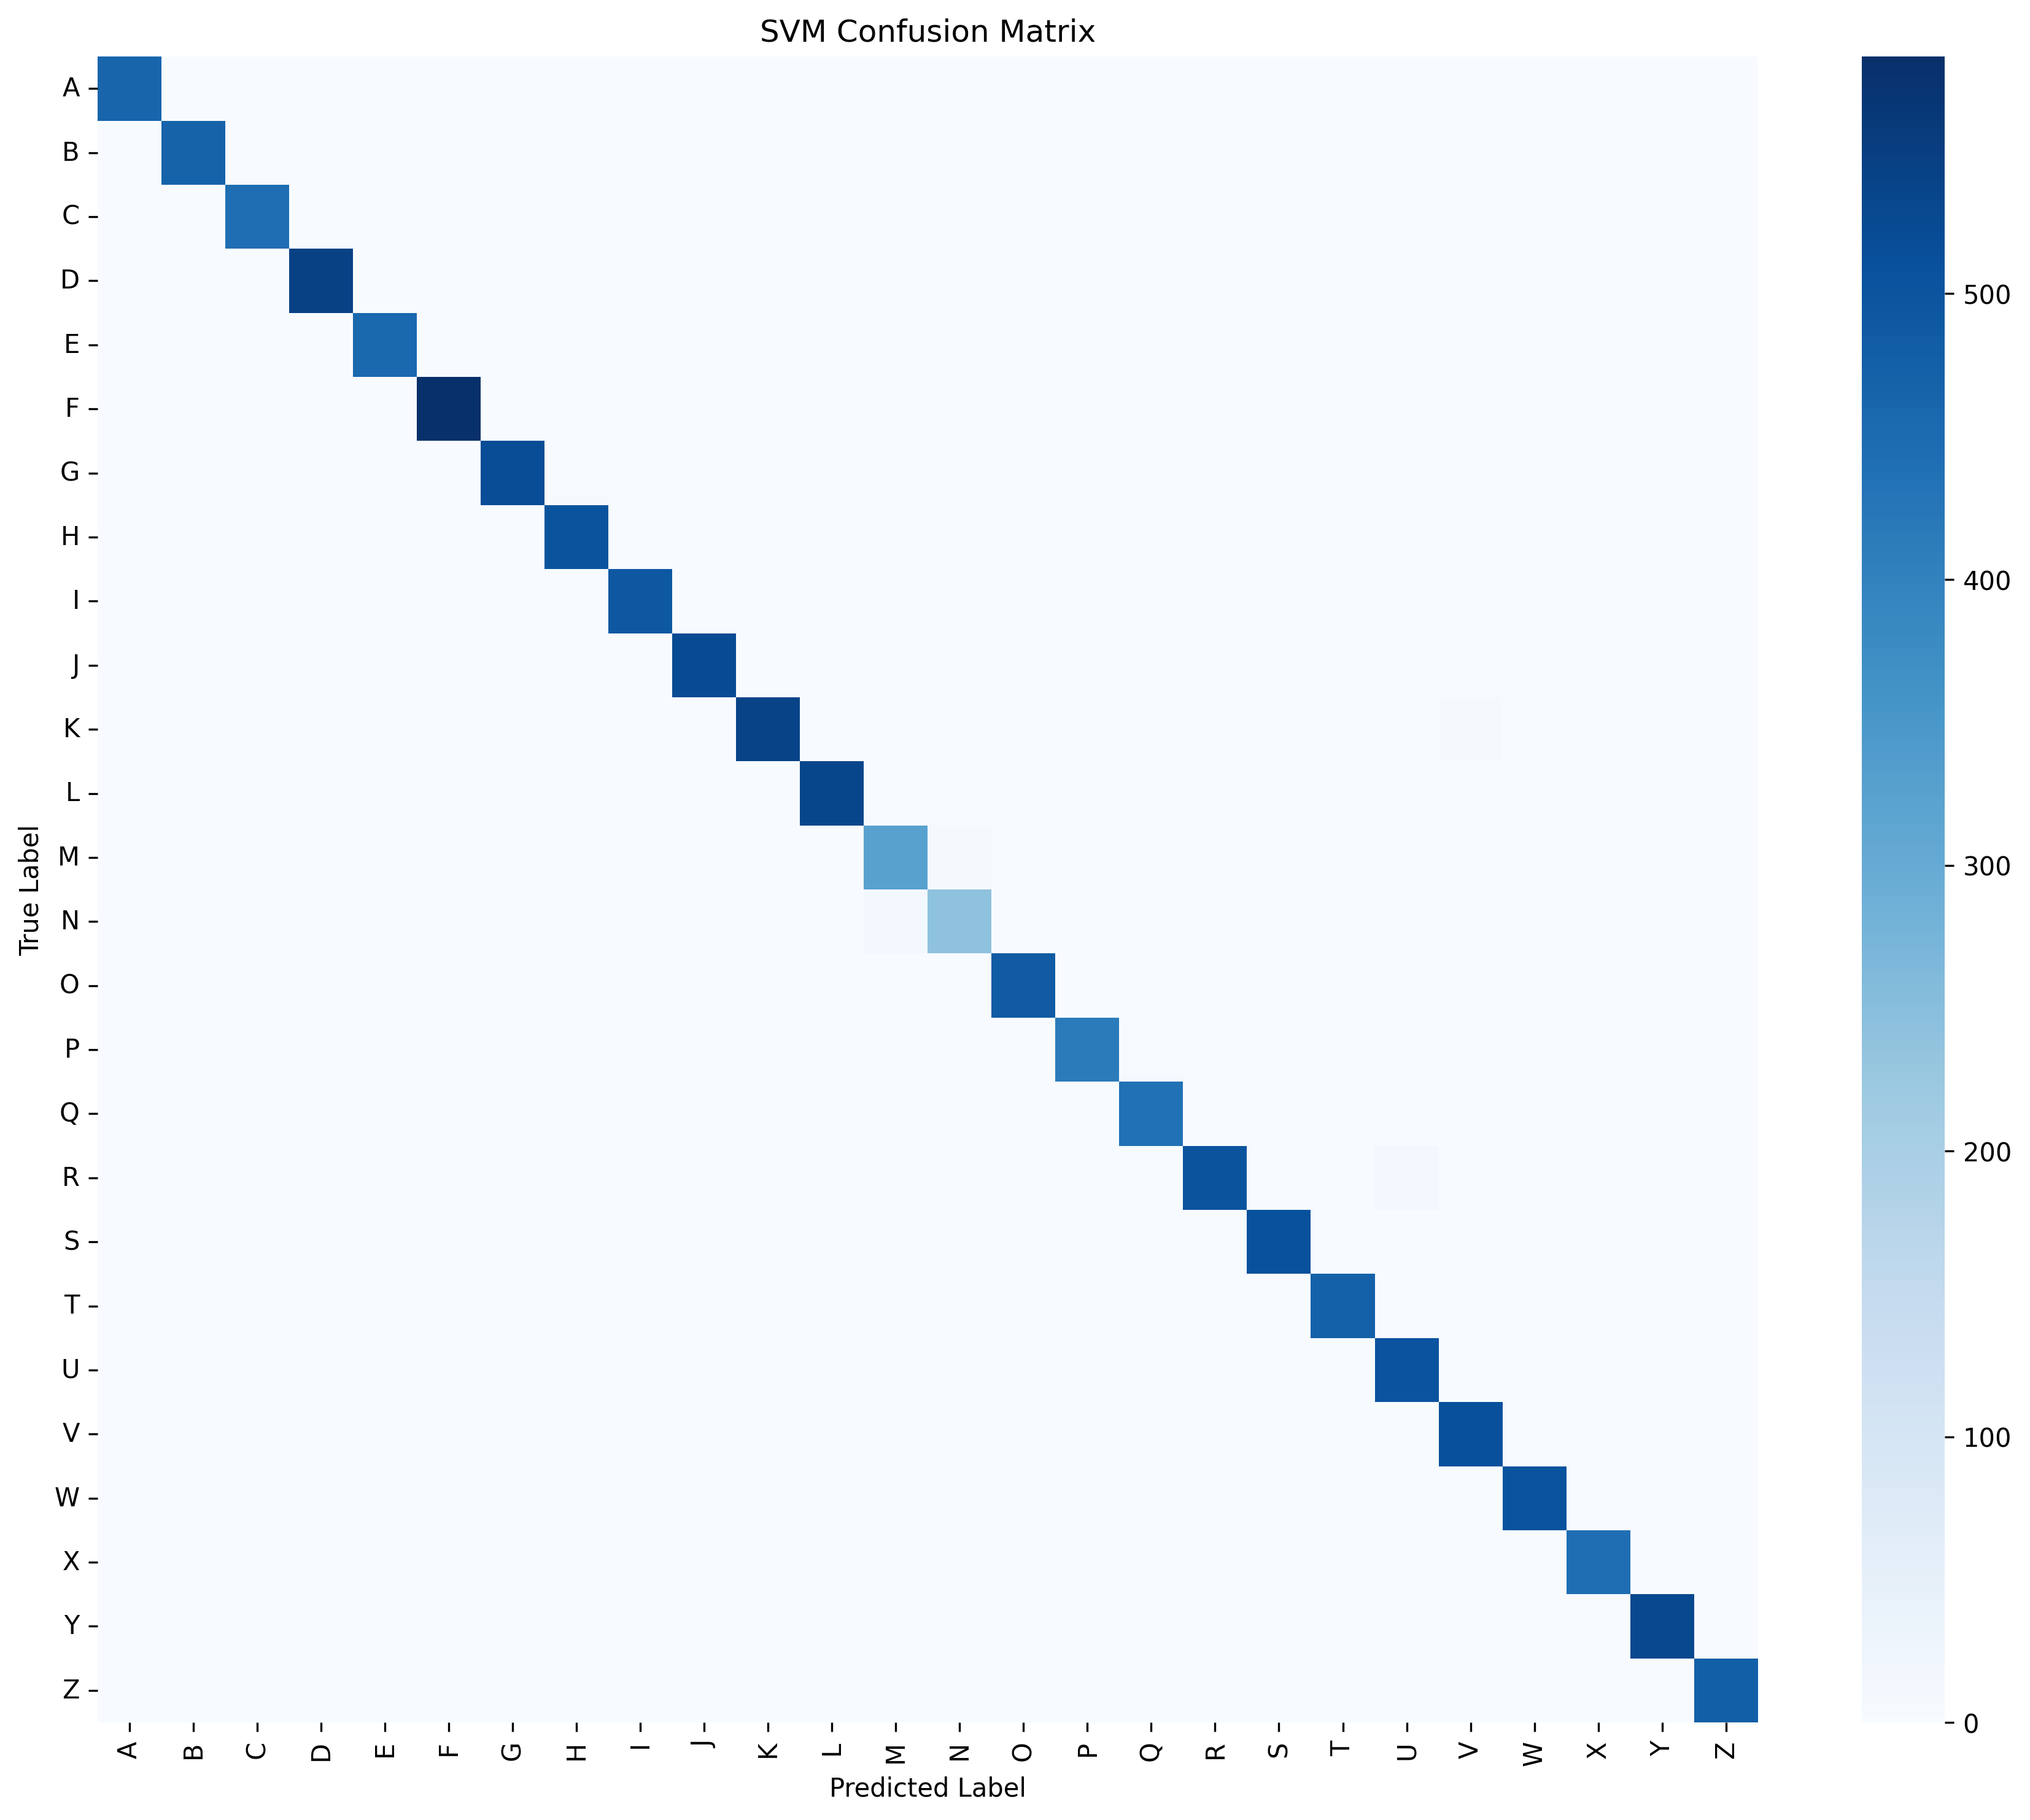
\includegraphics[width=0.75\linewidth]{images/SVM_confusion_matrix.png}
\end{figure}

Figure 1 shows a strong concentration of values along the diagonal, indicating that the majority of ASL alphabet gestures were correctly classified by the model. This demonstrates that the SVM classifier was highly effective in learning and distinguishing the spatial patterns derived from MediaPipe hand landmark coordinates. The high number of correct predictions across most classes confirms the reliability and robustness of the proposed approach for ASL gesture recognition.

Only minimal off-diagonal values were observed, suggesting that misclassifications occurred infrequently and were limited to a few visually similar hand gestures. These minor classification errors may be attributed to similarities in finger positioning and hand orientation between certain ASL letters, which can produce overlapping landmark patterns. Despite these challenges, the overall confusion matrix indicates that the SVM model maintained highly accurate and consistent predictions across the dataset.


\subsection{Feature Analysis and Importance of Hand Landmarks}

The extracted MediaPipe hand landmarks produced a structured 63-dimensional feature representation composed of the $(x, y, z)$ coordinates of 21 detected hand keypoints. These landmarks encoded the spatial arrangement of the wrist, finger joints, and fingertips, enabling the machine learning models to distinguish ASL alphabet gestures based on hand geometry rather than raw pixel information.

The high classification performance achieved by the SVM, Random Forest, and k-NN models indicates that the landmark features formed highly discriminative patterns within feature space. The SVM model achieved the highest overall accuracy of 98.8\%, suggesting that the extracted landmark coordinates provided sufficient spatial information for separating ASL classes with minimal overlap. Similarly, Random Forest and k-NN also achieved strong performance, indicating that the landmark representation effectively preserved gesture-specific structural characteristics.

The confusion matrix analysis further demonstrated the effectiveness of the extracted hand landmarks. Most predictions were concentrated along the diagonal of the confusion matrix, indicating that the landmark coordinates successfully captured the distinguishing spatial configurations of the ASL gestures. Misclassifications occurred only in a small number of visually similar letters, particularly among gestures such as M, N, R, U, and V. These classes involve subtle variations in finger positioning, overlap, and orientation, which can produce closely related landmark coordinate distributions.

The lower performance of Gaussian Naïve Bayes also highlighted the importance of spatial relationships among the landmark features. Unlike the other evaluated models, Naïve Bayes assumes feature independence, which is inconsistent with hand landmark data where finger and joint coordinates are strongly correlated. The significantly lower accuracy of Naïve Bayes suggests that the geometric dependencies between landmarks play a critical role in accurate ASL gesture recognition.